
\section{Identification of the boat parameters} \label{sec:part1}

\subsection{Transfer function from $\delta$ to $\psi$}
To start out this assignment we want to find the transfer function from $\delta$ to $\psi$, parameterized by T and K. By assuming no disturbances ($b=0$), the Laplace transformation of equation \cref{eq:psidot} and \cref{eq:rdot_def} give the following
\begin{equation}
    \mathscr{L}\{\ddot{\psi} = -\frac{1}{T}\dot{\psi} + \frac{K}{T}(\delta)\}
\end{equation}
\begin{equation*}
    \Rightarrow s^2\psi(s)+ s\psi(0) + \psi(0) + \frac{s}{T}\psi(s)+ \psi(0) = \frac{K}{T}\delta
\end{equation*}
and with the zero initial condition we find using.
\begin{equation} 
    H(s) =  \frac{\psi(s)}{\delta(s)} = \frac{K}{s(Ts+1)}
\end{equation}




\subsection{Parameters in smooth weather conditions}\label{1.b}
We now want to identify the parameters T and K in smooth weather conditions, this is with all disturbances turned off.  The input will be a sine function with amplitude 1 and frequency $\omega_1 = 0.005$ and $\omega_2 = 0.05$. 

\begin{figure}[H]
\begin{subfigure}{0.5\textwidth}
    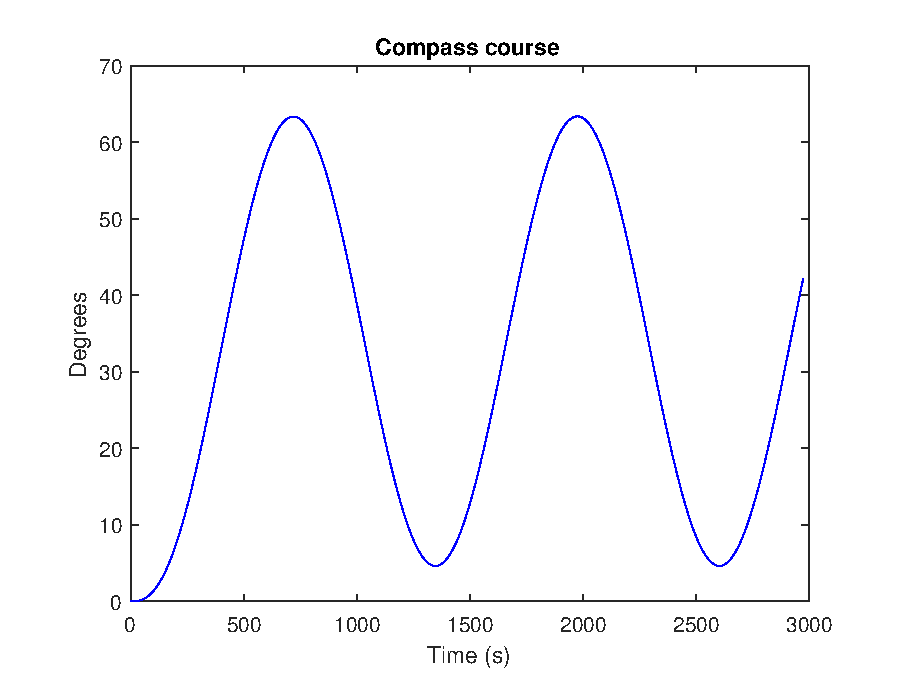
\includegraphics[width=1\linewidth]{Part1_pics/p1b_omega1.eps}
    \caption{$\omega_1$}
\end{subfigure}
\begin{subfigure}{0.5\textwidth}
    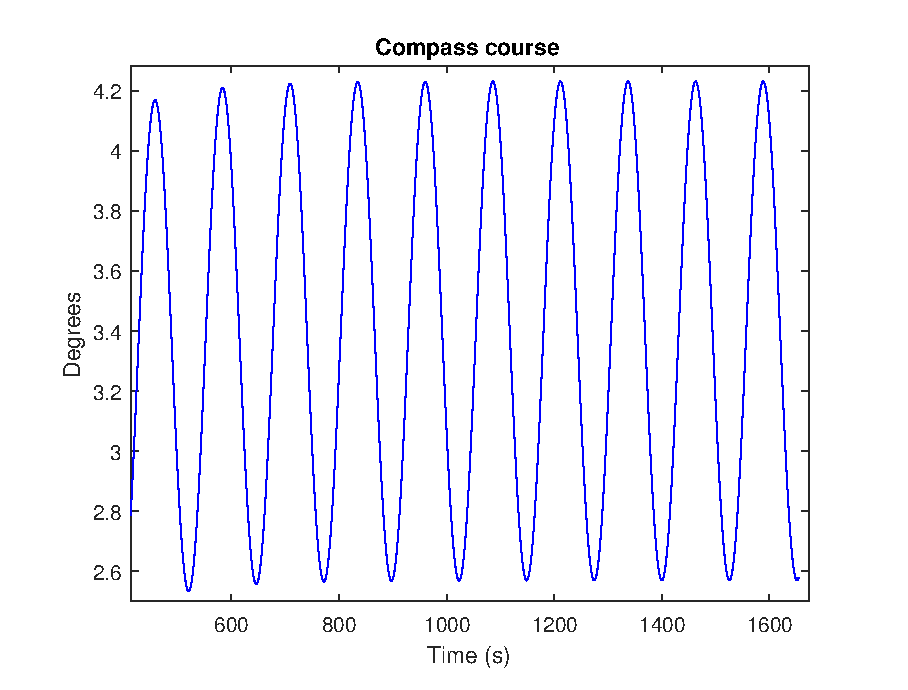
\includegraphics[width=1\linewidth]{Part1_pics/p1b_omega2_zoomedin.eps}
    \caption{$\omega_2$}
\end{subfigure}
\caption{Output of the Compass with $\omega_1$ and $\omega_2$}
\label{fig:p1b}
\end{figure}
After plotting the system, we calculated the average amplitude and got $A_1 = 29.354$ and $A_2 = 0.831$. 
This put us in a position so we culd solve the following equation for K and T.   
\begin{equation} \label{eq:transferfunction}
\begin{split}
    |H(j\omega)| &= \left| \frac{K}{j\omega(Tj\omega + 1)} \right| \\
    &= \frac{K}{\omega \sqrt{T^2 \omega^2 + 1}} \\
    &= A
\end{split}
\end{equation}
where $j = \sqrt{-1}$ for $\omega_1$ and $\omega_2$. From this we find by, isolating K, an expression for T
\begin{subequations}
\begin{equation}
    K = A_1 \omega_1 \sqrt{T^2 \omega_1 + 1} = A_2 \omega_2 \sqrt{T^2 \omega_2 + 1} \label{eq:K_def}
\end{equation}
\begin{equation}
    T^2 = \frac{A_2^2 \omega_2^2 - A_1^2 \omega_1^2}{A_1^2 \omega_1^4 - A_2^2 \omega_2^4} \label{eq:T_def}
\end{equation}
\end{subequations}
By changing the constants for their numbers the boat parameters are $T \approx 72.4264$ and $K \approx 0.1561$.





\subsection{Parameters with waves and measurement noise}
In this subsection we try to find the parameters K and T in rough weather condition. This means the wave and measurement noise are turned on. To solve this task we followed the same procedure as in the previous task.  
\bigskip
\begin{figure}[H]
    \centering
    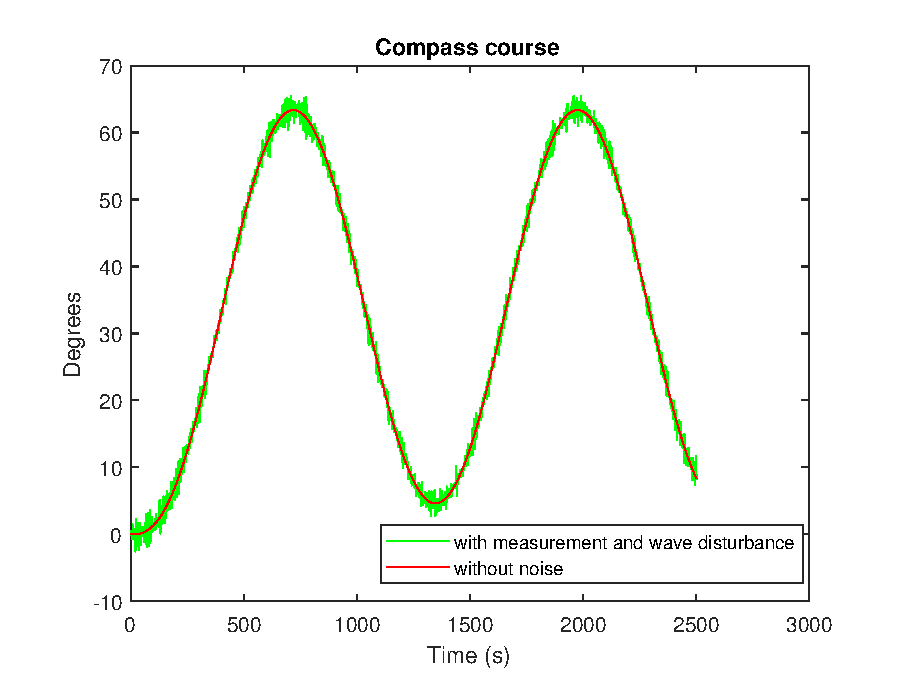
\includegraphics[width=0.75\linewidth]{Part1_pics/p1c_omega1_comp.eps}
    \caption{Compass comparison with $\omega_1$ and added noise, $\omega_1$= 0.005}
    \label{fig:p1c1}
\end{figure}
For finding the average amplitude: 
\begin{equation*}
    A_{1,1} = \frac{65.34 - 2.702}{2} = 31.344
\end{equation*}
\begin{equation*}
    A_{1,2} = \frac{65.47 - 2.495}{2} = 31.4875
\end{equation*}
The average of $A_{1,1}$ and $A_{1,2}$ then becomes 31.41575. With the noise added to the model it will not be possible to obtain equally good estimations as it was in the previous task.  This because it is more challenging to get the right values for the amplitude.
\begin{figure}[H]
    \centering
    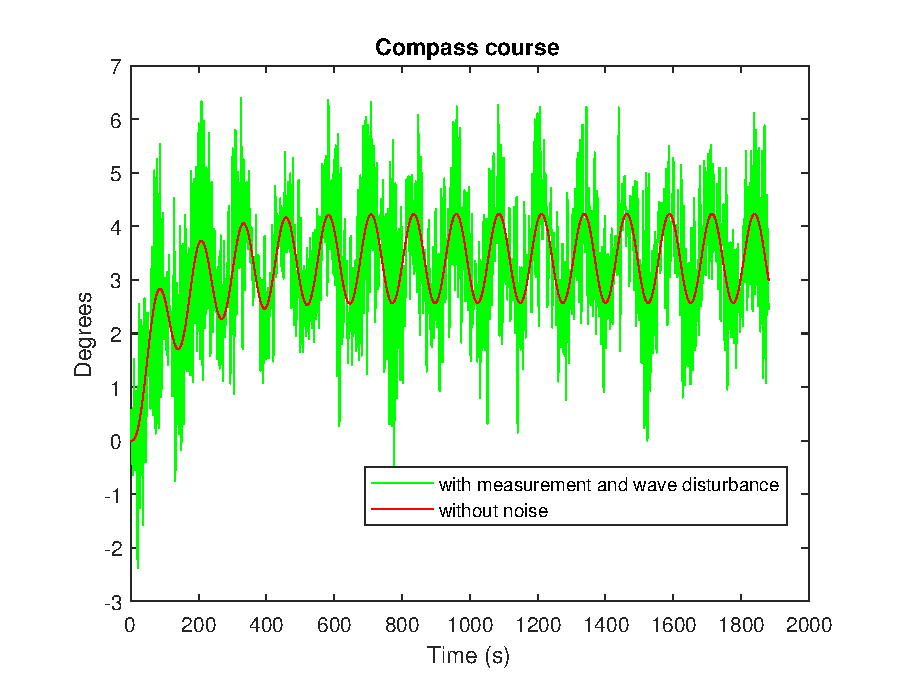
\includegraphics[width=0.75\linewidth]{Part1_pics/p1c_omega2_comp.eps}
    \caption{Compass comparison with $\omega_2$ and added noise}
    \label{fig:p1c2}
\end{figure}
For $\omega$= 0.05 it is nearly impossible to approximate good parameters. \Cref{fig:p1c2} shows how difficult it is to separate the noise from the desired signal. This will not make the model a good approximation of the ship. 
\newline
A solution for this is to run the signals through a low-pass filter before finding the values for the parameters. After trying to find the average so that we can find a value for the amplitude we got
\begin{equation*}
    A_{1,1} = \frac{5.384 - 1.942}{2} = 1.721
\end{equation*}
\begin{equation*}
    A_{1,2} = \frac{6.36 - 1.451}{2} = 2.4545
\end{equation*}
\begin{equation*}
    A_{1,3} = \frac{6.321 - 0.2752}{2} = 3.0229
\end{equation*}
Giving the average for $A_1$ as 2.39946 which gave $T_c = 290.67$ and $K = 0.1576$. The new T varied quite a bit from section \ref{1.b}. So we can conclude that tuning the ship in rough weather conditions is not ideal.  


\subsection{Step response}
For testing how good the approximation is, a step input of 1 degree to the rudder at t = 0 is implemented. See \cref{sim:part1d} in \cref{sec:simulink_diagrams} for the simulink implementation.
\begin{figure}[H]
    \centering
    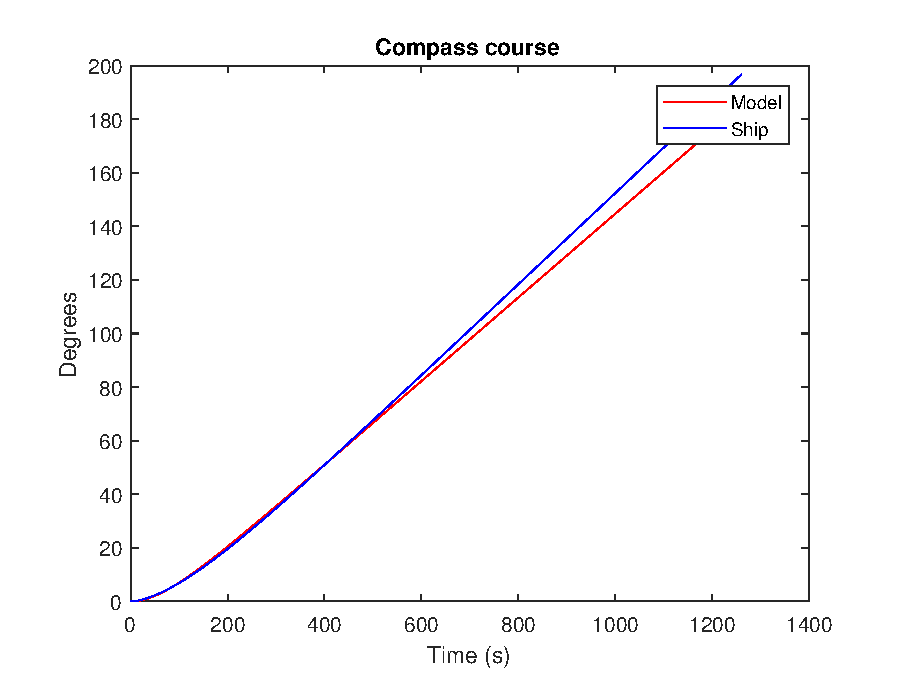
\includegraphics[width=0.8\linewidth]{Part1_pics/p1d.eps}
    \caption{Step response of the model compared to the step response of the ship }
    \label{fig:p1d}
\end{figure}
The comparison tells us that the model are close to the ship in the fist 600 second. But after this the difference of the models increases. The bigger the deviations, will result in a non optimal regulator. The design we have bean using is for an optimized regulator. 
\bigskip
The result is acceptable, because an approximation will never exactly be like the original system. 



